\documentclass[mathserif]{beamer}
\usetheme[secheader]{pecostalk}
\graphicspath{{figs/}}                                                                                                                              

\usepackage{mhchem}
\usepackage{hyperref}

\newcommand{\abs}[1]{\ensuremath{ \left|#1\right|}}
\newcommand{\bt}[1]{{\ensuremath{\boldsymbol{#1}}}}
\newcommand{\bv}[1]{{\ensuremath{\boldsymbol{#1}}}}
\newcommand{\commentout}[1]{}
\newcommand{\ds} {\; d\Gamma}
\newcommand{\dx} {\; d\Omega}
\newcommand{\grad}[1]{\bv{\nabla} {#1}}
\newcommand{\norm}[1]{\ensuremath{ \left|\left|#1\right|\right|}}
\newcommand{\orderof}[1]{\ensuremath{ {\cal O}\left(#1\right)}}
\newcommand{\pdv}[2]{\frac{\partial #1}{\partial #2}}

\newcommand{\UQ}[1]{{\color{red}{#1}}}

\newcommand{\adjointsol}{{\ensuremath{\bv{\tilde{z}}}}}
\newcommand{\adjointsolh}{{\ensuremath{\bv{\tilde{z}^h}}}}
\newcommand{\adjointsolH}{{\ensuremath{\bv{\tilde{z}^H}}}}
\newcommand{\param}{{\ensuremath{\xi}}}
\newcommand{\params}{{\ensuremath{\bv{\param}}}}
\newcommand{\primalsol}{{\ensuremath{\bv{\tilde{u}}}}}
\newcommand{\primalsolh}{{\ensuremath{\bv{\tilde{u}^h}}}}
\newcommand{\primalsolH}{{\ensuremath{\bv{\tilde{u}^H}}}}
\newcommand{\Res}{{\ensuremath{\mathcal R}}}
\newcommand{\Qoi}{{\ensuremath{Q}}}


\newcommand{\software}[1]{{\texttt{#1}}}
\newcommand{\libMesh}{\software{libMesh}}
\newcommand{\PETSc}{\software{PETSc}}
\newcommand{\GRINS}{\software{GRINS}}
\newcommand{\cpp}{\software{C++}}




\date{February 27, 2017}
\author[R. Stogner]{Roy H. Stogner}

\institute{The University of Texas at Austin}
\title[libMesh]{libMesh: Past, Present, and Future}

\AtBeginSection[]{\frame{\tableofcontents[current]}}

\begin{document}
\begin{frame}
\begin{center}

\includegraphics[width=.8\linewidth]{grand_logo}\\
\end{center}
\titlepage
\begin{flushright}
%
\includegraphics[scale=0.1]{asc_logo}\\
\end{flushright}
\end{frame}

%   \begin{frame}
%       \frametitle{Outline}
%       \tableofcontents
%   \end{frame}

\section{Community}


%===============================================================================
% NEW SLIDE
%===============================================================================
\begin{frame}{libMesh Community}
\begin{columns}
\column{.4\textwidth}
\begin{block}{Scope}
\begin{itemize}
\item Free, Open source
\begin{itemize}
\item LGPL2 for core
\end{itemize}
\item 45 Ph.D.\ theses, 507 papers (81 in 2015)
\item $\sim10$ current developers
\item $110-240$ current users?
\end{itemize}
\end{block}

\column{.6\textwidth}
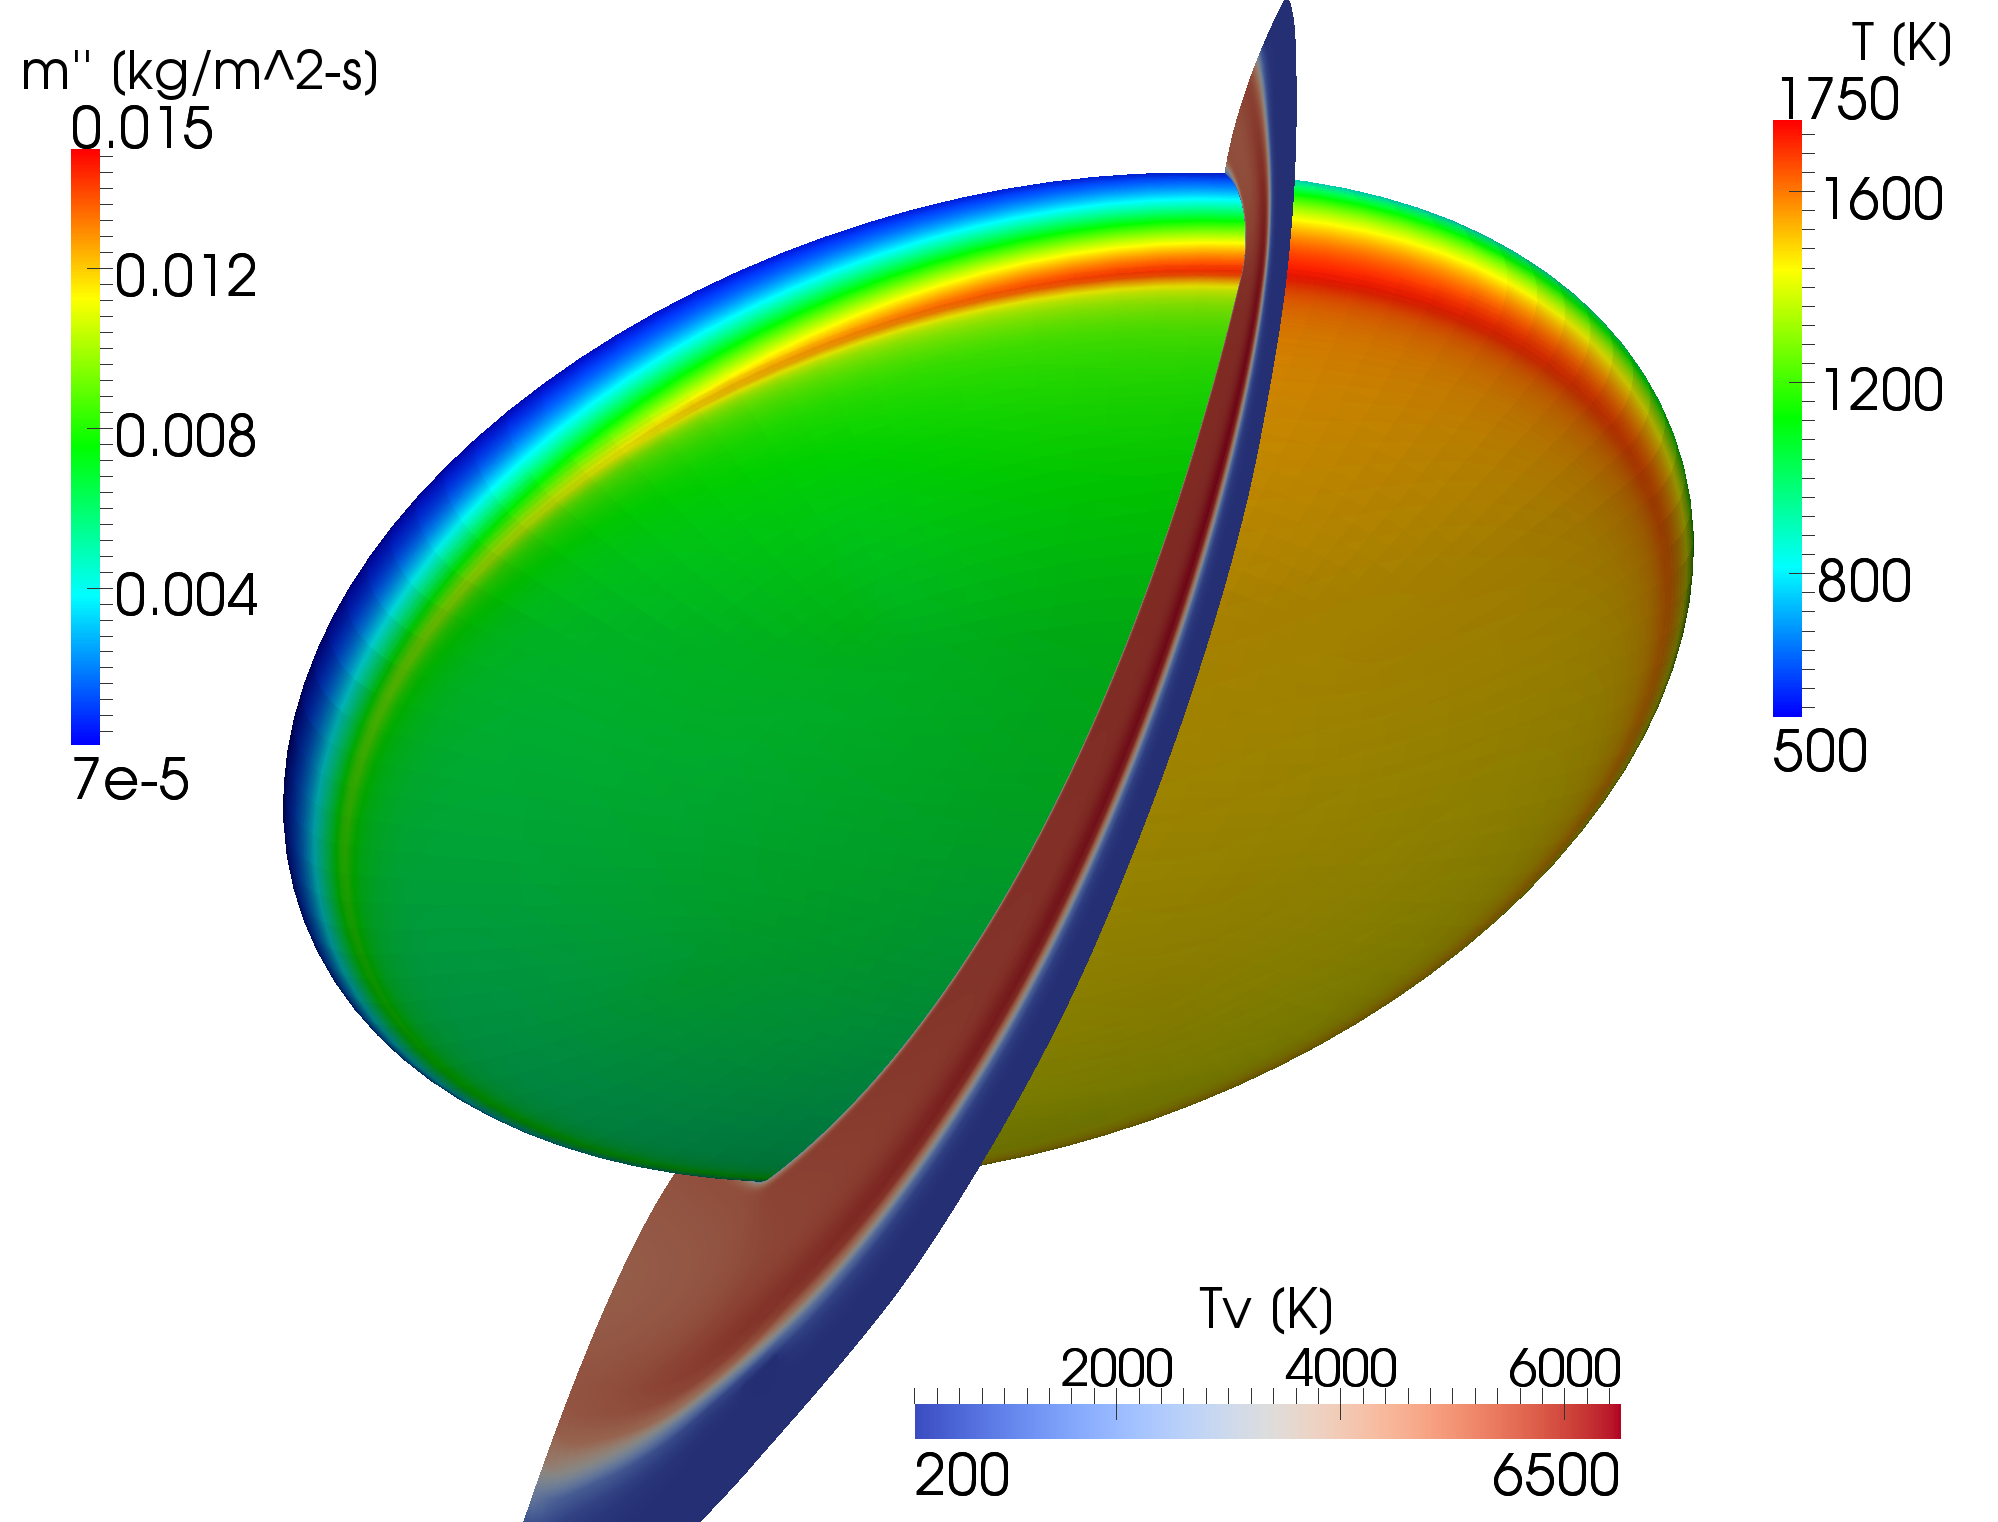
\includegraphics[width=.45\textwidth]{ablating_hs_wbg}
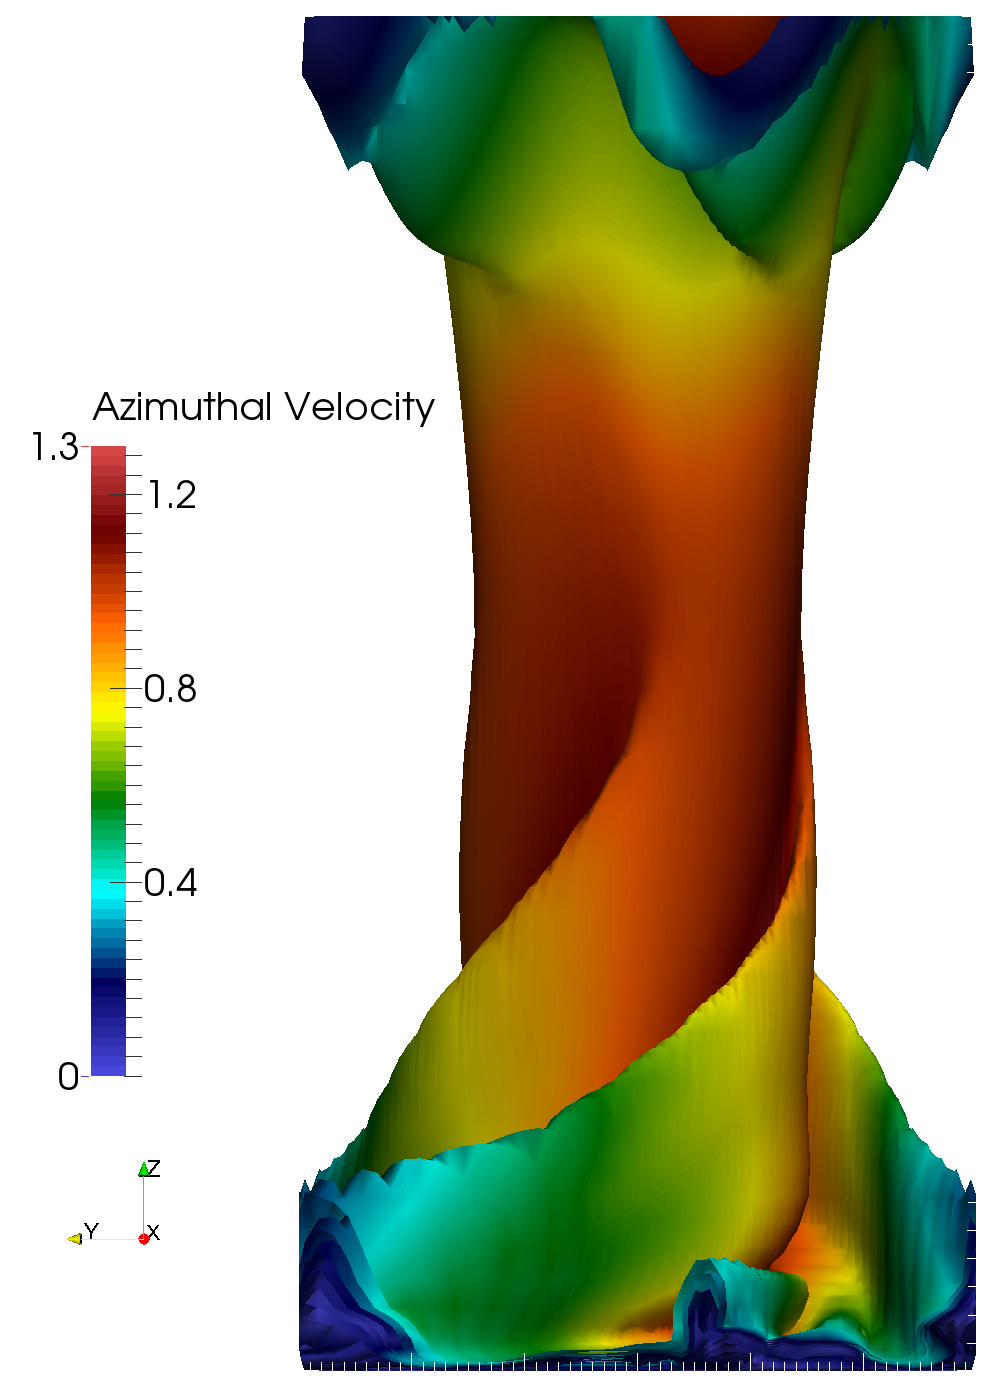
\includegraphics[width=.25\textwidth]{sov}
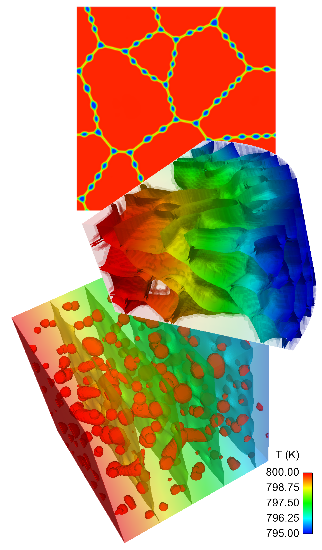
\includegraphics[width=.3\textwidth]{marmot1b}
\end{columns}

\begin{columns}
\column{.35\textwidth}
\includegraphics[width=\textwidth]{libmesh_citations}

\column{.65\textwidth}
\begin{block}{Challenges}
\begin{itemize}
\item Radically different application types
\item Widely dispersed core developers
\begin{itemize}
\item INL, UT-Austin, U.Buffalo, JSC, MIT, Harvard, Argonne
\end{itemize}
\item OSS, commercial, private applications
\end{itemize}
\end{block}
\end{columns}

\end{frame}



%===============================================================================
% New Slide
%===============================================================================
\begin{frame}
\frametitle{\GRINS}

\begin{block}{\url{https://github.com/grinsfem/grins}}
  \begin{itemize}
  \item Multiphysics FEM platform built on \libMesh{}
  \item Modular structure for ``Physics'', solvers, QoIs, etc.
  \item Key feature: automatically enabled discrete adjoints (AMR, sensitivities)
  \end{itemize}
\end{block}

\begin{columns}[T]
  \begin{column}{0.4\textwidth}
    \centerline{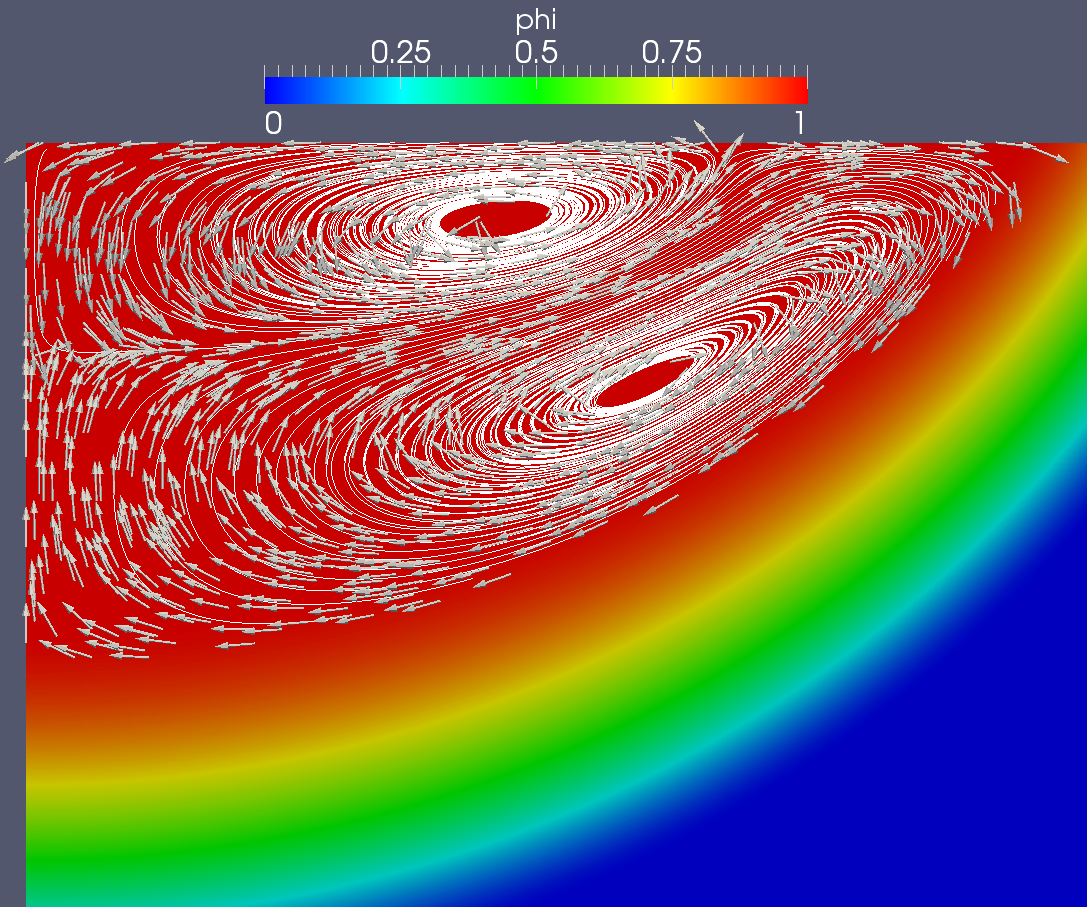
\includegraphics[width=\linewidth]{var_vortices}}
  \end{column}
  %
  \begin{column}{0.4\textwidth}
    \centerline{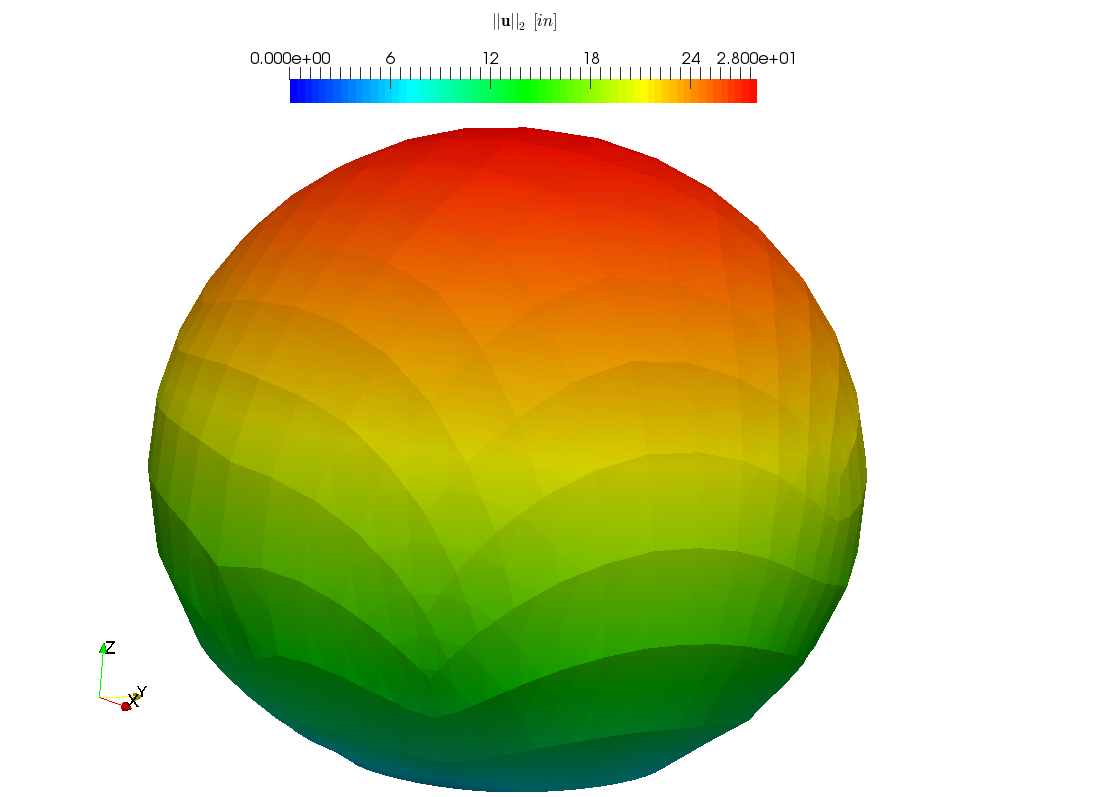
\includegraphics[width=\linewidth]{balloon_4}}
  \end{column}
  %
  \begin{column}{0.2\textwidth}
    \centerline{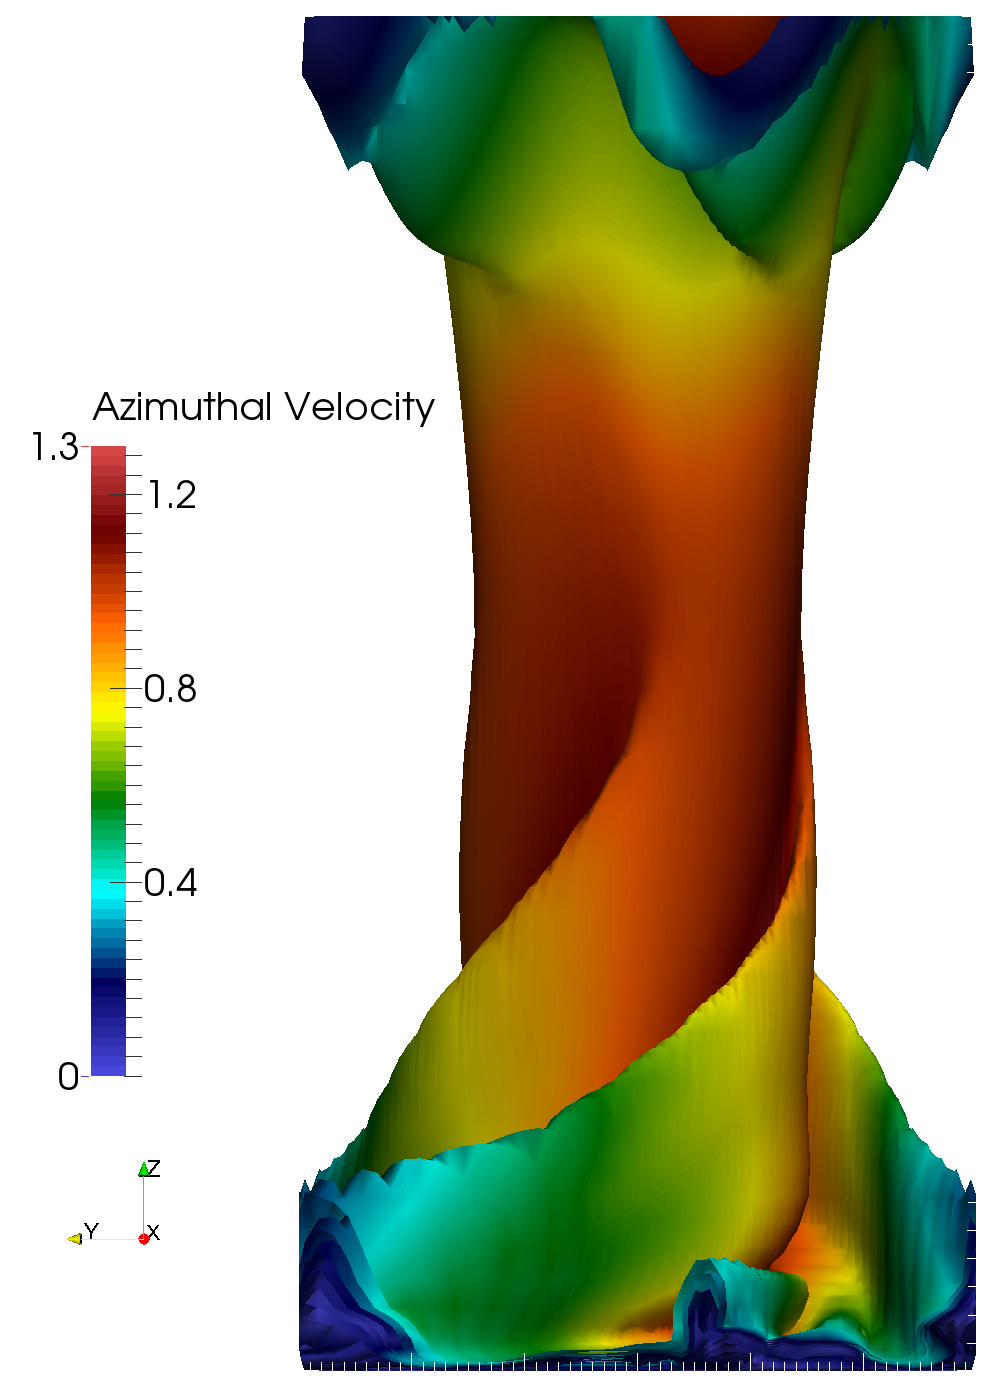
\includegraphics[width=\linewidth]{sov}
    \tiny{Courtesy Nick Malaya, UT Austin}}
  \end{column}
  \end{columns}

\end{frame}



\frame
{
  \frametitle{The MOOSE Framework - Gaston et al., INL}
  \begin{center}
    \fbox{\includegraphics[page=2,height=0.8\textheight]{Gaston/talk}}
  \end{center}
}





\section{Design Philosophy}

%===============================================================================
% NEW SLIDE
%===============================================================================
\begin{frame}
\frametitle{Modular Programming}
\begin{columns}
\begin{column}{.35\textwidth}
\begin{center}
\includegraphics[width=\textwidth]{modular_fem}
\end{center}
\end{column}
\begin{column}{.65\textwidth}
\begin{block}{Discrete Components, Interfaces}
\begin{itemize}
\item Linear, nonlinear solvers are discretization-independent
\item System assembly, solution I/O \& postprocessing can be
discretization-independent
\item Time, space discretizations can be physics-independent
\item Some error analysis, sensitivity methods can be
physics-independent
\end{itemize}
\end{block}

\begin{itemize}
\item Reusable components get re-tested

\item Errors too subtle to find in complex physics are easy to spot
in benchmark problems.
\end{itemize}
\end{column}
\end{columns}

\end{frame}


%===============================================================================
% NEW SLIDE
%===============================================================================
\begin{frame}
\frametitle{Object Oriented Programming}
\begin{columns}
\begin{column}{.55\textwidth}
\begin{block}{ABC: Abstract Base Class}
\begin{itemize}
\item One abstract interface
\item Many instantiations
\item Hides derived type from most uses
\end{itemize}
\end{block}

Example: Geometric elements
\begin{itemize}
\item Base classes give DoF indexing, mesh topology
\item Instantiations give mesh geometry
\item Most Mesh code is element-independent
\end{itemize}
\end{column}
\begin{column}{.45\textwidth}
\begin{center}
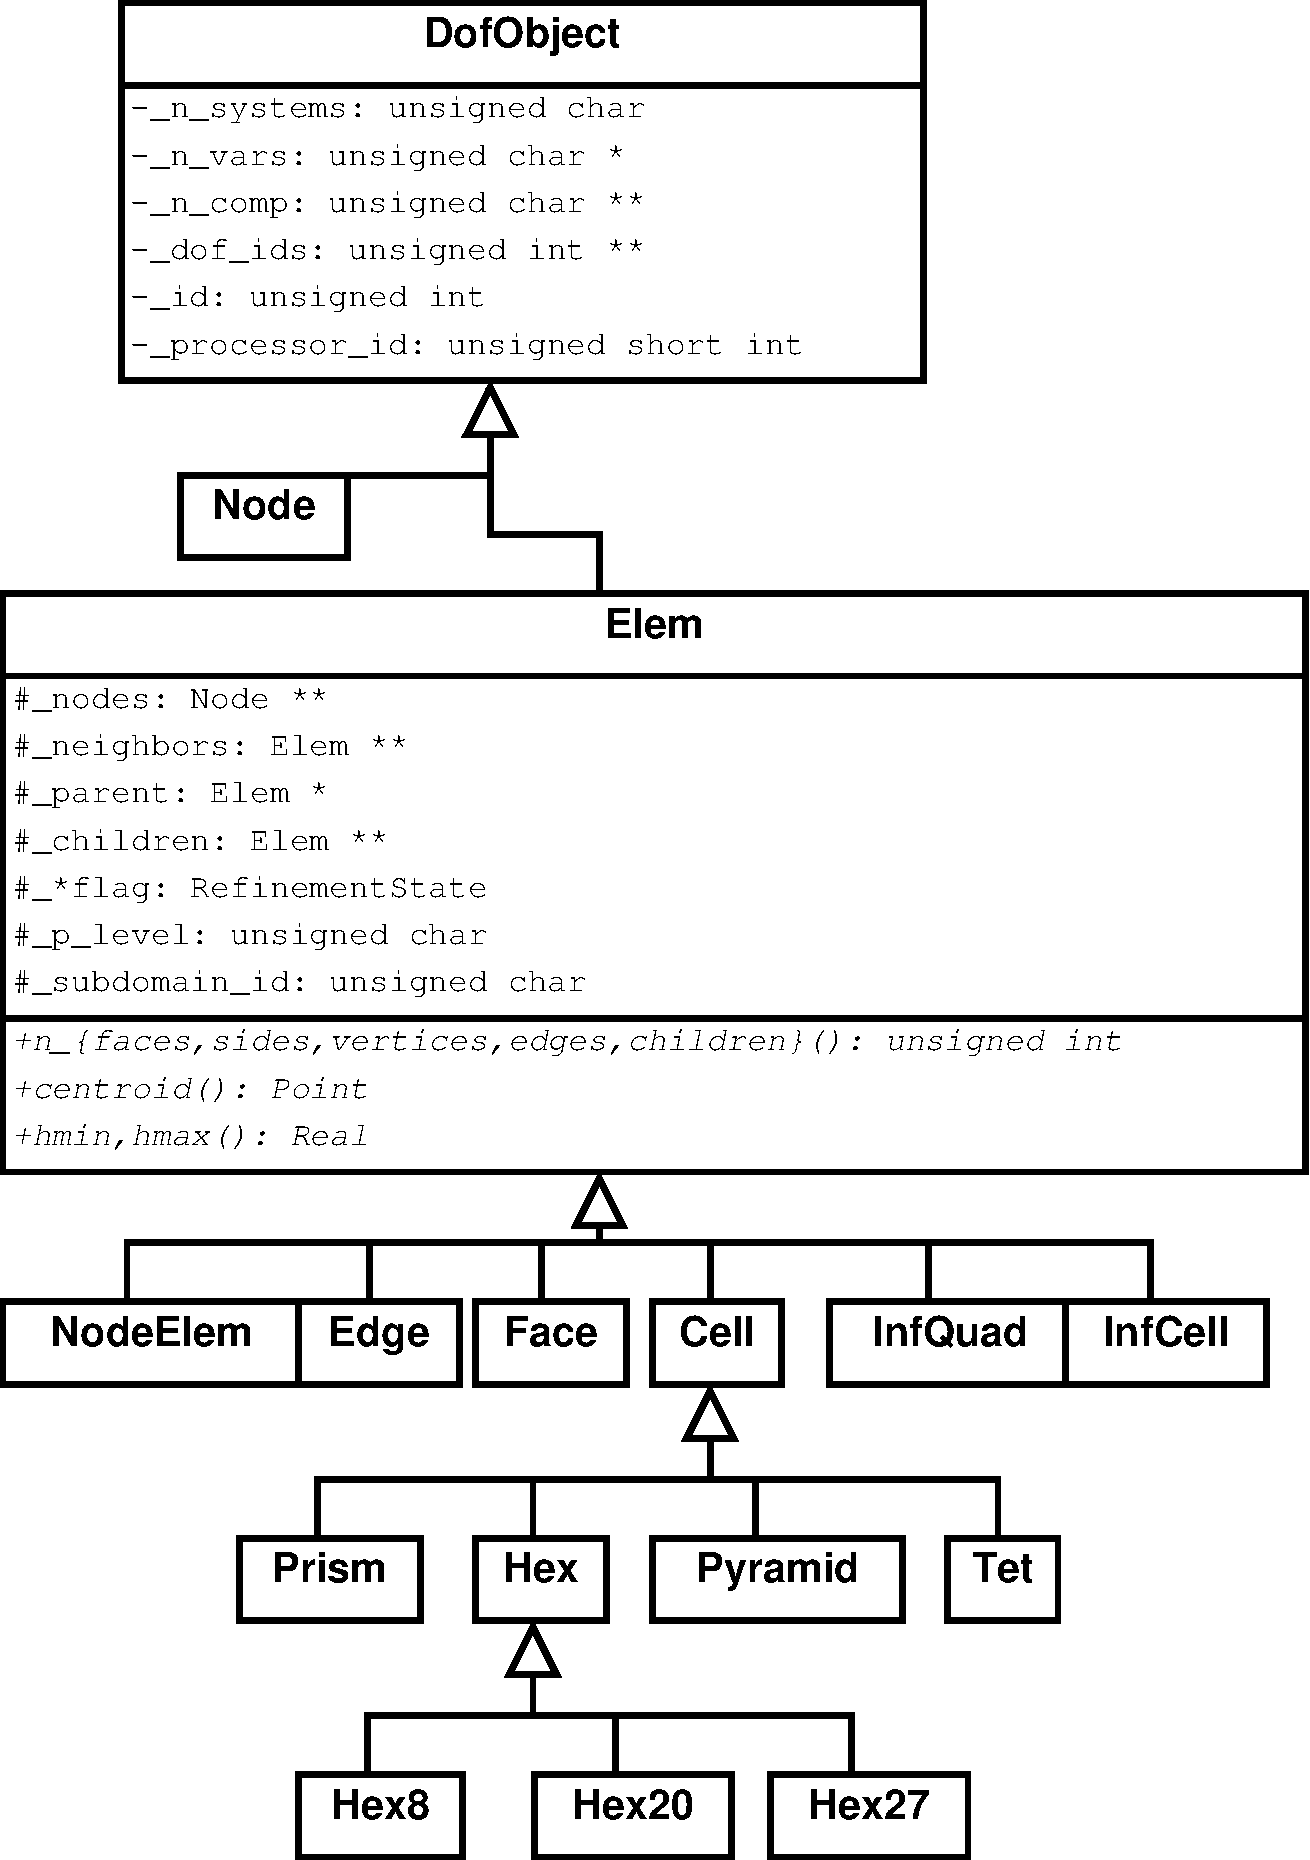
\includegraphics[width=.95\textwidth]{DofObjects}
\end{center}
\end{column}
\end{columns}

\end{frame}


%===============================================================================
% NEW SLIDE
%===============================================================================
\begin{frame}
\frametitle{Software Reuse}
\begin{columns}
\begin{column}{.4\textwidth}

\begin{itemize}
\item Don't reinvent the wheel unnecessarily!

\item Time spent rewriting something old is time that could have been spent
writing something new.

\item More eyes == fewer bugs

\item Extensions interoperate
\end{itemize}
\end{column}
\begin{column}{.6\textwidth}
\begin{center}
\includegraphics[width=.8\textwidth]{fins_modules}
\end{center}
\end{column}
\end{columns}

\end{frame}

\section{Distributed Collaboration}

%===============================================================================
% NEW SLIDE
%===============================================================================
\begin{frame}
\frametitle{Collaboration Styles}

\begin{columns}
\begin{column}{.6\textwidth}

How does collaborative \libMesh{} discussion and development take place?

\pause

\begin{itemize}[<+->]
    \item Yelling at the guy on the other side of the CFDLab
    \item User, developer mailing lists
    \item libMesh, MOOSE, GRINS issue trackers
    \item Private email?  Instant messaging?  Videoconferencing?
\end{itemize}

\end{column}
\begin{column}{.4\textwidth}

\visible<3->{
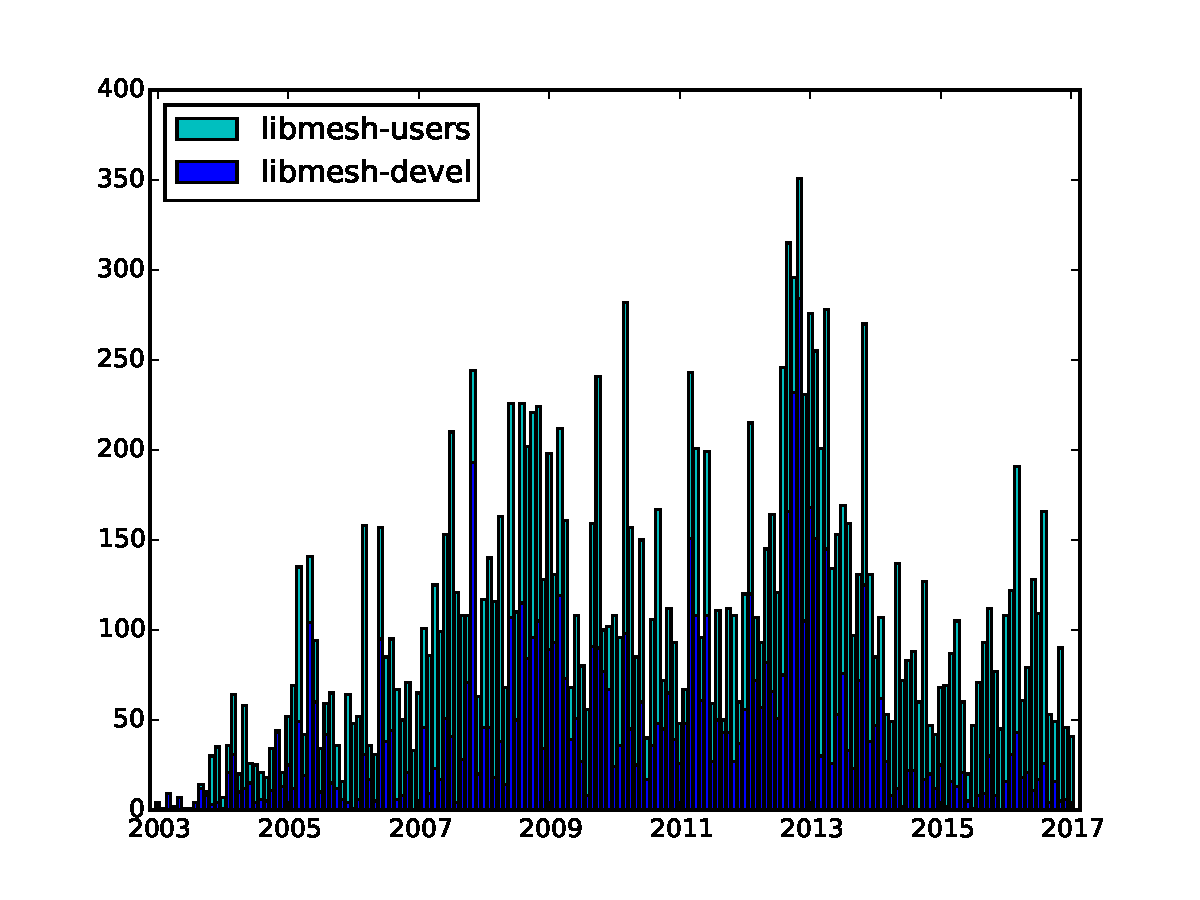
\includegraphics[width=\textwidth]{libmesh_mailinglists}
}

\visible<4->{
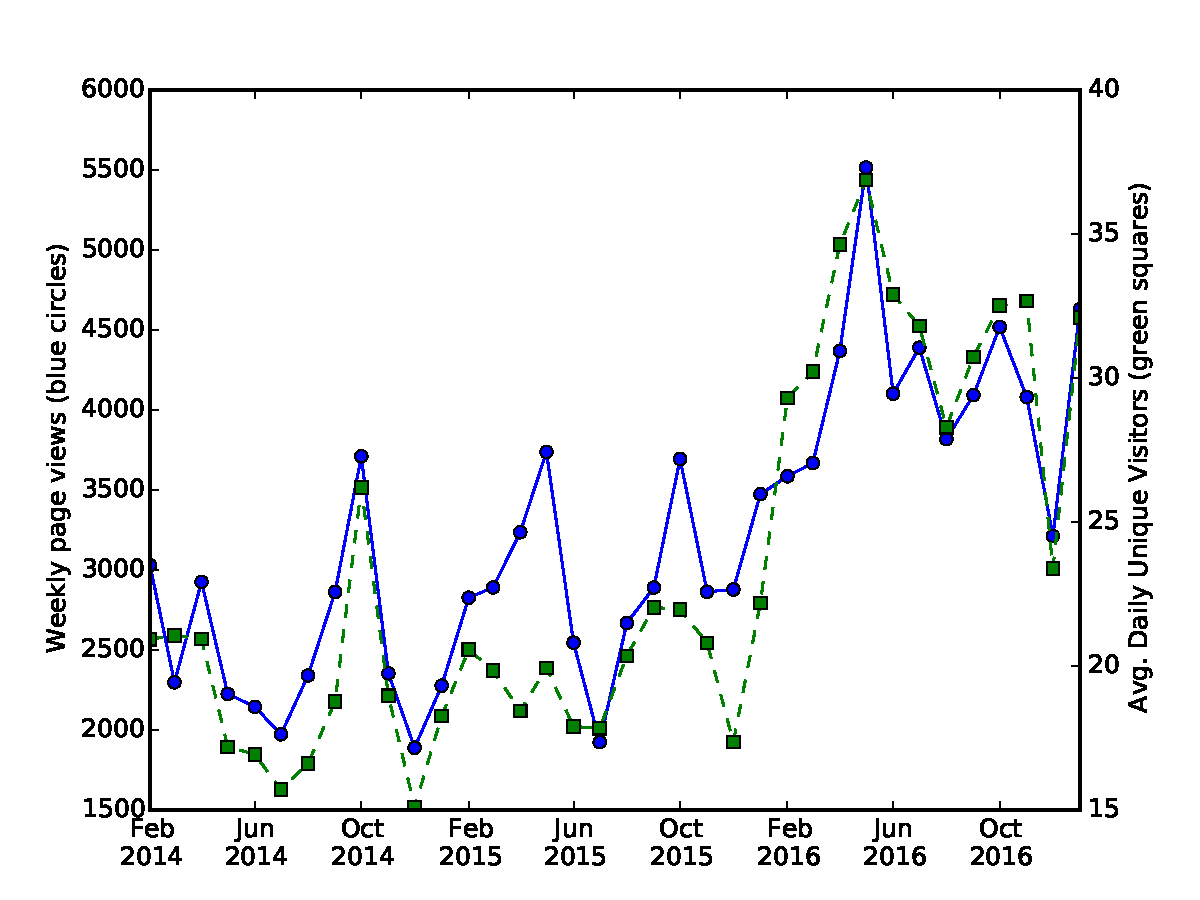
\includegraphics[width=\textwidth]{monthly_github_traffic}
}

\end{column}
\end{columns}
\end{frame}


%===============================================================================
% NEW SLIDE
%===============================================================================
\begin{frame}[fragile]
\frametitle{Tracking API Changes}

\begin{block}{API versions easily proliferate...}
%\begin{minted}[fontsize=\footnotesize]{c++}
\small
\begin{semiverbatim}
#if PETSC_VERSION_LESS_THAN(3,1,0)
  ierr = MatGetSubMatrix(matrix->mat(),
           _restrict_to_is, _restrict_to_is_complement,
           \alert{PETSC_DECIDE}, MAT_INITIAL_MATRIX, &submat1);
#else
  ierr = MatGetSubMatrix(matrix->mat(),
           _restrict_to_is, _restrict_to_is_complement,
           MAT_INITIAL_MATRIX, &submat1);
#endif
\end{semiverbatim}
%\end{minted}
\end{block}

\begin{itemize}
	\item Maintain a wide range of external compatibility
        \begin{itemize}
            \item Dropped PETSc 2.3.3 (2007) support for libMesh 1.0 (2016)
            \item C++11 shims
        \end{itemize}
	\item Limit \libMesh{} API changes
\end{itemize}

\end{frame}

\begin{frame}
\frametitle{Signaling API Changes}
\begin{block}{Development practices}
\begin{itemize}
	\item Old, new APIs {\emph{overlap}}
	\item Easier with C++ function overloading, default arguments
	\begin{itemize}
		\item Adding \texttt{f(a,b)} does not preclude keeping
			\texttt{f(a)}
		\item Adding \texttt{f(a,b=default)} can replace
			\texttt{f(a)}
	\end{itemize}
\end{itemize}
\end{block}

\begin{block}{Runtime warnings}
\begin{itemize}
	\item {\texttt{libmesh\_experimental()}} \quad (in-flux APIs)
	\item {\texttt{libmesh\_deprecated()}} \quad ($\sim$1 year, 1-2 releases)
\end{itemize}
\end{block}

\begin{block}{Examples}
\begin{itemize}
	\item {\texttt{OStringStream} workaround class}
	\item {\texttt{Parallel::} global functions}
\end{itemize}
\end{block}


\end{frame}



%===============================================================================
% NEW SLIDE
%===============================================================================
\begin{frame}
\frametitle{Verification}

    Does everyone's interpretation of API {\emph{semantics}} match?

\pause

\vfill

``When in trouble when in doubt, run in circles scream and shout.''\\
- old Army War College football team slogan

\pause

{\texttt{
\\
\#if IN\_DOUBT \{ \\
\quad if (in\_trouble()) \{ \\
\quad\quad  run\_in\_circles(); // Stack traces, data printing \\
\quad\quad  scream\_and\_shout(); // Exception throw \\
\quad \} \\
\#endif
}}

\pause

{\texttt{
\\
assert(!in\_trouble());
}}

\pause

\begin{itemize}
\item Each new assertion becomes a new ``contract''
\end{itemize}

\end{frame}

%===============================================================================
% NEW SLIDE
%===============================================================================
\begin{frame}[fragile]
\frametitle{High-level Assertions}
\begin{block}{{\texttt{libmesh\_assert()}, \PETSc} debug mode}
\begin{itemize}
\item Function preconditions - are arguments all valid?
\item Function postconditions - is result valid?
\item Active in ``debug'' or ``devel'' runs
\item Approx. 7000 asserts in \libMesh{}; more in GRINS, MOOSE
\end{itemize}
\end{block}

\pause

{\footnotesize
\begin{verbatim}
libmesh_assert(neigh->has_children());
libmesh_assert(this->initialized());
libmesh_assert((ig >= Ug.first_local_index()) &&
               (ig < Ug.last_local_index()));
libmesh_assert(requested_ids[p].size() == ghost_objects_from_proc[p]);
libmesh_parallel_only(mesh.comm());
MeshTools::libmesh_assert_valid_node_procids(mesh);
libmesh_assert(error_estimator.error_norm.type(var) == H1_SEMINORM ||
               error_estimator.error_norm.type(var) == W1_INF_SEMINORM)
libmesh_assert(number_h_refinements > 0 || number_p_refinements > 0);
\end{verbatim}
}
\end{frame}



\section{Future Design Directions}


%===============================================================================
% NEW SLIDE
%===============================================================================
\begin{frame}
\frametitle{Upgraded DistributedMesh Support}
\begin{columns}
\column{.6\textwidth}
\begin{center}
\includegraphics[width=.95\textwidth]{MeshUML}
\end{center}
\column{.4\textwidth}
%\begin{block}{}
\begin{itemize}
\item \texttt{MeshBase} gives node or element iterators
\item \texttt{ReplicatedMesh} or \texttt{DistributedMesh} manages synchronized or distributed data
\item Redistribution, AMR/C, etc handled via library
\end{itemize}

\includegraphics[width=.75\textwidth]{ParallelMesh3}
%\end{block}
\end{columns}

\end{frame}


%===============================================================================
% NEW SLIDE
%===============================================================================
\begin{frame}[fragile]
\frametitle{Physics via C++14 Generic Programming}

\begin{itemize}
\item {\textbf{C++98:}} intrusive metaprogramming

\begin{semiverbatim}
template <typename T1, typename T2, typename T3>
typename PlusType<typename MultipliesType<T1,T2>::type,
                  typename ExpType<T3>::type>::type
f(const T1& m, const T2& x, const T3& b)
\{ return m*x+exp(b); \}
\end{semiverbatim}

\item {\textbf{C++14:}} user-friendly return type deduction

\begin{semiverbatim}
template <typename T1, typename T2, typename T3>
auto f(const T1& m, const T2& x, const T3& b)
\{ return m*x+exp(b); \}
\end{semiverbatim}

\end{itemize}

\end{frame}



%===============================================================================
% NEW SLIDE
%===============================================================================
\begin{frame}[fragile]
\frametitle{Physics via C++14 Generic Programming}

\begin{itemize}

\item Expression-template-compatible kernels:

\begin{semiverbatim}
template <typename ContextType,
          typename CacheType>
auto weak_interior_residual
  (const ContextType& context,
   const CacheType&) const
  \{
    auto& du_dx  = std::get<1>(context.u);
    auto& v_vals = std::get<0>(context.v);

    return _b*du_dx*v_vals;
  \}
\end{semiverbatim}

\item \software{Eigen::Array} calculations auto-vectorize

\item \software{vex::vector} calculations run on GPU

\item \software{MetaPhysicL::DualExpression} calculations provide Jacobian too

\end{itemize}

\end{frame}



%===============================================================================
% NEW SLIDE
%===============================================================================
\begin{frame}[fragile]
\frametitle{Geometric Multigrid Support}

\begin{itemize}

    \item Leverage PETScDM interface for solver infrastructure
    \item libMesh provides mesh hierarchies, prolongation and
        restriction operators between meshes
    \item Future API for user-specified projection operators
    \item Applicable to any libMesh-based application compiled with PETSc

\end{itemize}

      \begin{tabular}{l*{6}{c}r}
        Number of Levels  & 2 & 3 & 4 & 5 & 6  & 7 & 8 \\
        \hline
        1-D Laplace & 4 & 4 & 8(,2) & 9(,2) & 9(,2) & 9(,2) & 9(,2)\\
        2-D Laplace (Quads) & 5 & 5 & 5 & 5 & 5 & 5 & 5  \\
        3-D Laplace (Hexes) & 4 & 5 & 6 & 6 & 5 & 5 & -  \\
        2-D Laplace (Tris) & 5 & 7 & 7 & 7 & 7 & 7 & 7  \\
        3-D Laplace (Tets)  & 6 & 8 & 9 & 9 & - & - & -  \\
      \end{tabular}

      \vspace{1em}
      (,2) indicates a second outer solver iteration

\end{frame}



\section{Acknowledgements}

%===============================================================================
% NEW SLIDE
%===============================================================================
\begin{frame}
\frametitle{Acknowledgements}

Recent \libMesh{} contributors:
\begin{columns}

\column{.45\textwidth}

\begin{itemize}
\item David Andrs
\item Paul Bauman
\item Vikram Garg
\item Derek Gaston
\item Dmitry Karpeev
\end{itemize}

\column{.45\textwidth}
\begin{itemize}
\item Benjamin Kirk
\item David Knezevic
\item Cody Permann
\item John Peterson
\item Sylvain Vallaghe
\end{itemize}

\end{columns}

\vspace{5mm}

Useful resources:
\begin{itemize}
\item libMesh: \url{https://libmesh.github.io/}
\item MOOSE: \url{https://mooseframework.org/}
\item GRINS: \url{https://grinsfem.github.io/}
\end{itemize}

\vspace{5mm}

Dr.\ Graham F.\ Carey: "No one ever got a Ph.D.\ from here for writing
a code."

\end{frame}

\end{document}
